\documentclass[12pt] {article}
\usepackage{cmap}
\usepackage[T2A]{fontenc}
\usepackage[utf8]{inputenc}
\usepackage{ifluatex}
\usepackage{svg}
\usepackage{enumerate}
\usepackage{hyperref}
\usepackage{mathtools}

\usepackage{geometry}
 \geometry{
 a4paper,
 total={210mm,297mm},
 left=20mm,
 right=20mm,
 top=20mm,
 bottom=20mm,
 }

\usepackage[english,russian]{babel}
\usepackage{graphicx}
\usepackage{listings}

\title{Летучка 2.}

\begin{document}
\clearpage
\thispagestyle{empty}
\begin{enumerate}
\item Что такое cross-fold validation? 
\vspace{10mm}
\item Какой гипотезой мы руководствуемся, чтобы построить метрический классификатор? Сформулировать.
\vspace{10mm}
\item ${a(u, X^l) = \arg\max_{y \in Y} \underbrace{\sum\limits_{i=1}^l [y_u^i = y]w(i, u)}_{\Gamma_y(u)} }$\\
\\ Смысл параметров $w$, $i$, $u$, $\Gamma_y(u)$
\vspace{10mm}
\item Мотивация для использования Парзеновского окна. В чем минусы зависимости веса объекта только от его порядкового номера?
\vspace{10mm}
\item Какими свойствами должна обладать функция $K$, чтобы использовать ее в качестве ядра?
\vspace{10mm}
\item 
\begin{minipage}[t]{0.65\linewidth}
      Что по оси ординат? 
   \end{minipage}%
   \hfill
   \begin{minipage}[t]{0.35\linewidth}
     %\centering
     \vspace{-9.5ex}
	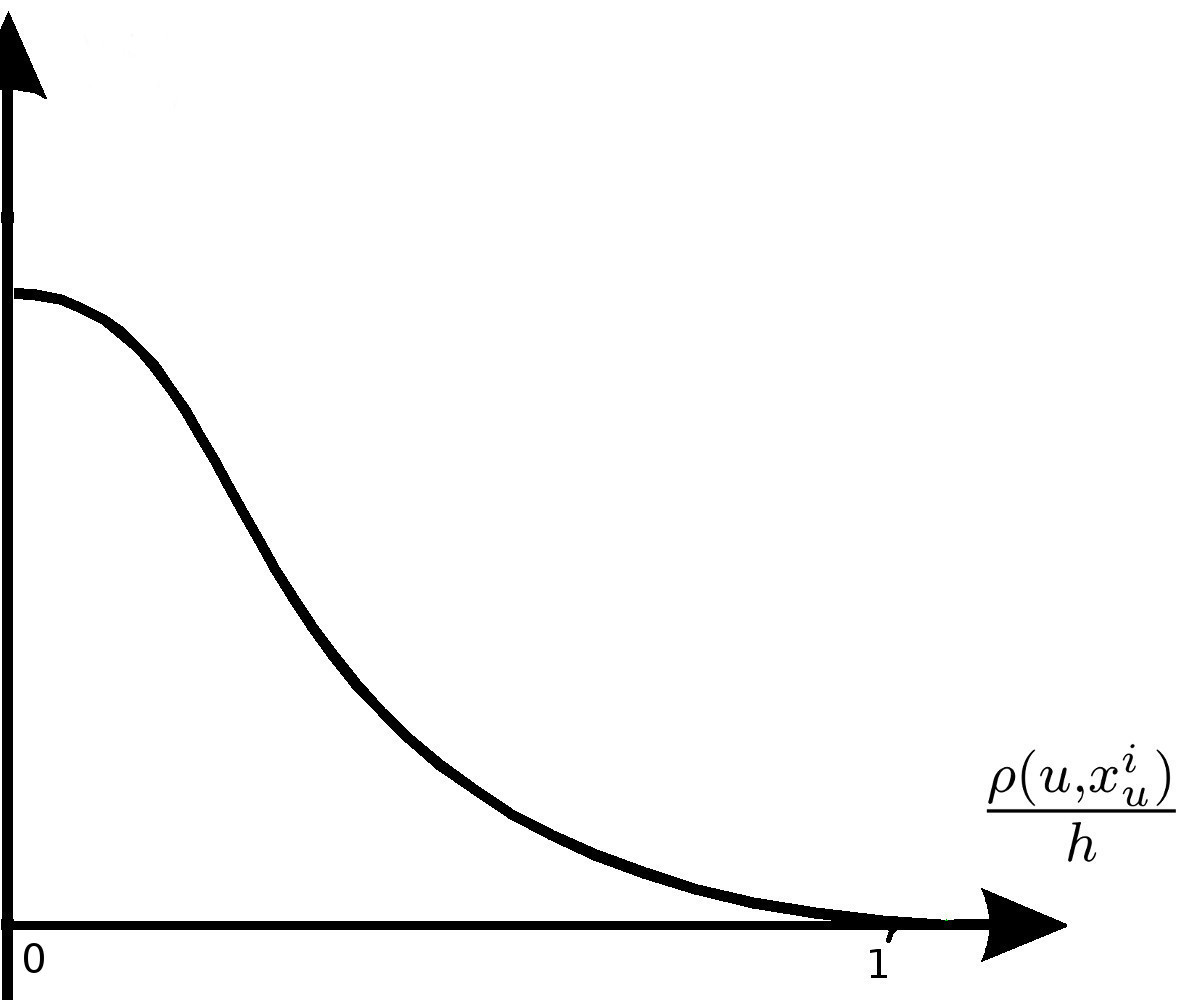
\includegraphics[width=.9\textwidth]{parzen}
   \end{minipage}
   
\item \begin{minipage}[t]{0.65\linewidth}
      Как подбирать функцию расстояния? 
   \end{minipage}%
\vspace{10mm}
\item Что такое проклятие размерности?
\vspace{10mm}
\item Жадное добавление признаков -- как определить, что признаков уже достаточно?
\vspace{10mm}
\item Чем эталонный объект отличается от надежно классифицируемого?

\end{enumerate}

\end{document}
